%!TEX root = ../thesis.tex
%*******************************************************************************
%*********************************** Introduction Chapter *****************************
%*******************************************************************************
\chapter*{Introduction}
\addcontentsline{toc}{chapter}{Introduction}
\chaptermark{Introduction}
%********************************** %First Section  **************************************


%============================================================%
%============================================================%
\section*{Industrial context and motivation}
%============================================================%
%============================================================%

The shift in wind energy projects from limited onshore resources to the vast potential of offshore locations is a growing trend. 
Offshore wind energy offers several advantages, including more consistent winds and the ability to install larger turbines
Since the installation of the first offshore wind farm in Vindeby, Denmark, in 1991, the industry has experienced rapid growth, with a total capacity of 56GW exploited worldwide in 2021. 
Over time, offshore wind technology has matured, resulting in significant achievements such as securing projects in Europe through "zero-subsidy bids," where electricity generated by wind farms is sold at wholesale prices. 

However, despite the progress of this sector, scaling limitations emerge and numerous scientific challenges.
To meet ambitious national and regional development targets, the wind energy industry must address various scaling issues, including port logistics, the demand for critical natural resources, and sustainable end-of-life processes. 
Furthermore, the field presents various scientific challenges that often involve coupling data with numerical simulations of physical systems and their surrounding environment.
The wind energy community is focused on several objectives, including enhancing the design of floating offshore wind turbines, refining wind resource estimation techniques, and optimizing maintenance operations. 
Additionally, the design, installation and exploitation of these industrial assets implicate several decision-making steps, considering limited access to information.
Therefore, properly modeling and treating the various uncertainties along this process proved to be a key success factor in this highly competitive industry.

%The design of an offshore wind farm depends on multiple site parameters such as the water depth, soil properties, wind, waves and currents conditions, and the local community acceptance. 
%Fortunately, international standards regulate this activity and provide general engineering guidelines. 

Overall, the industry needs methods and techniques for uncertainty management to optimize safety margins and asset management
As a wind farm project developer, the attention is first drawn to refining the wind potential of candidate sites by combining different sources of information and 
modeling the multivariate distribution of environmental conditions within a wind farm. 
In floating projects, the probabilistic design helps to define safer and more robust solutions. 
As a wind farm owner, another significant consideration revolves around end-of-life management. 
This involves evaluating three possible outcomes: extending the operating assets' lifetime, replacing current turbines with more advanced models, or dismantling and selling the wind farm. 
The first two solutions require assessing the current reliability of the structure and its remaining useful life. 
These quantitative evaluations are studied by certification bodies and insurance providers to issue exploitation permits.
To deliver rigorous risk assessments, the generic \textit{uncertainty quantification methodology} may be adopted.

%============================================================%
%============================================================%
\section*{Generic methodology for uncertainty quantification}
%============================================================%
%============================================================%

Uncertainty Quantification (\acrshort{UQ}) aims at modeling and managing uncertainties in complex systems.
Over the year, generic UQ frameworks were proposed \elias{add ref Deroc.} to quantify and analyze the relations between uncertain input factors and the systems' outcomes. 
UQ is particularly relevant in situations where experiments or direct observations are costly, time-consuming, or even impossible to conduct.

Computer experiments, also known as numerical experiments or simulations, play an important role in UQ. 
They involve the use of numerical models to simulate the behavior of a system under various conditions and parameter settings. 
These virtual experiments provide a cost-effective way to explore the behavior of complex systems and make robust and well-informed decisions.
They enable researchers and decision-makers to gain a deeper understanding of the system dynamics, optimize designs, assess risk, and make robust predictions. 
As a result, uncertainty quantification has become an essential tool in wind energy, benefiting from the multiphysics numerical models simulating the behavior of wind farms interacting with their environment.
Nevertheless, numerical models should be calibrated against measured data and pass validation, and verification processes \elias{add ref} to minimize the residual modeling error.
Figure \ref{fig:UQ_methodo} illustrates the UQ methodologies and the standardized usual steps encountered during a study, which are detailed hereafter: 
\begin{itemize}
    \item \textbf{Step A -- Problem specification}: at this step, it is necessary to establish the system under study and construct a numerical model capable of precisely simulating its behavior.
    Specifying the problem also involves defining the complete set of parameters inherent to the computer model. 
    This includes the input variables as well as determining the specific output quantity that will be generated by the numerical model;
    \item \textbf{Step B -- Uncertainty modeling}: The objective of the second step is to identify all the sources of uncertainty impacting the input variables.
    Most of the time choosing a probabilistic framework, the modeling methods will depend on the available information (e.g., amount of data, input dimension);
    \item \textbf{Step C -- Uncertainty propagation}: This step consists in propagating the uncertain inputs through the computer model, making the output uncertain. 
    Then, the goal becomes the estimation of a quantity of interest (i.e., a statistic on the random output variable of interest).
    The uncertainty propagation method may differ depending on the quantity of interest targeted (e.g., central tendency, rare event);    
    \item \textbf{Step C' -- Inverse analysis}: In this additional step, a sensitivity analysis can be performed to study the role allocated to each uncertain input leading to the uncertain output;    
    \item \textbf{Metamodeling}: Since this methodology is frequently used with computationally expensive numerical models, it becomes interesting to emulate these models using statistical models constructed from a limited number of simulations.
    The uncertainty quantification is then performed on the so-called ``metamodel'' (or surrogate model) at a reasonable computation cost.
\end{itemize}


\begin{figure}[!h]
    \centering
    %\begin{figure}[h]
%    \centering
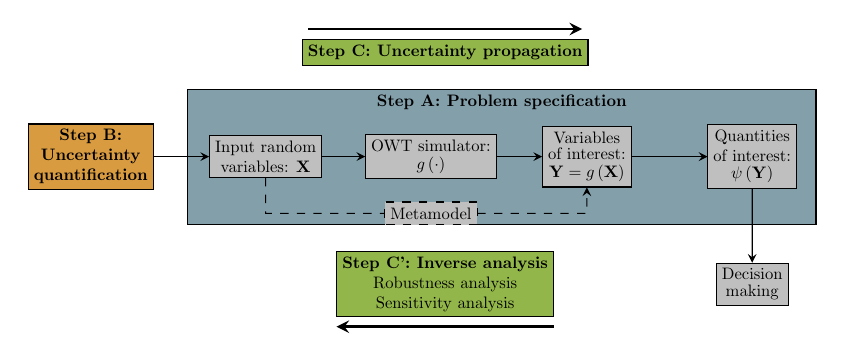
\begin{tikzpicture}[scale=0.6, every node/.style={transform shape}]
    \node[rectangle,draw,fill=YellowOrange!70!gray] (a) at (-9,0) {\shortstack{\textbf{Step B:} \\ \textbf{Uncertainty} \\ \textbf{quantification}}};
\node[rectangle,draw,fill=YellowGreen!70!gray] (f) at (-1.5,2.2) {
\textbf{Step C: Uncertainty propagation}};
\node[rectangle,draw,fill=YellowGreen!70!gray] (g) at (-1.5,-2.7) {\shortstack{
\textbf{Step C': Inverse analysis} \\ Robustness analysis \\ Sensitivity analysis}};
\node[rectangle,draw,minimum width=13.3cm,fill=SkyBlue!40!gray] (h) at (-0.3,0) {\shortstack{\textbf{Step A: Problem specification} \\ \phantom{a} \\ \phantom{a} \\ \phantom{a} \\ \phantom{a} \\ \phantom{a} \\ \phantom{a} \\ \phantom{a} \\ \phantom{a} \\ \phantom{a} }};
\node[rectangle,draw,fill=lightgray] (b) at (-5.3,0) {\shortstack{
Input random \\ variables: $\mathbf{X}$}};
\node[rectangle,draw,fill=lightgray] (c) at (-1.8,0) {\shortstack{
OWT simulator: \\$g\left(\cdot\right)$}};
\node[rectangle,draw,fill=lightgray] (d) at (1.5,0) {\shortstack{
Variables \\ of interest: \\ $\mathbf{Y}=g\left(\mathbf{X}\right)$}};
\node[rectangle,draw,fill=lightgray] (e) at (5,0) {\shortstack{
Quantities \\ of interest: \\ $\psi \left(\mathbf{Y}\right)$}};
\node[rectangle,draw,fill=lightgray, dashed] (i) at (-1.8,-1.2) {Metamodel};
\node[rectangle,draw,fill=lightgray] (j) at (5,-2.7) {\shortstack{Decision \\ making}};
\draw[-stealth, black, line width=1pt] (-4.4,2.7) -- (1.4,2.7);
\draw[-stealth, black, line width=1pt] (0.8,-3.6) -- (-3.8,-3.6);
\draw[-stealth, black] (a) -- (b);
\draw[-stealth, black] (b) -- (c);
\draw[-stealth, black] (c) -- (d);
\draw[-stealth, black] (d) -- (e);
\draw[-stealth, black, dashed] (b) -- (-5.3,-1.2) -- (i) -- (1.5,-1.2) -- (d);
 \draw[-stealth, black] (e) -- (j);

\end{tikzpicture}
%    \caption{General uncertainty quantification and propagation framework}
%    \label{Fig:UQ}
%\end{figure}
    \caption{General uncertainty quantification framework (adapted from \cite{ajenjo_2023}) \elias{remove maths and add image?}}
    \label{fig:UQ_methodo}
\end{figure}


%============================================================%
%============================================================%
\section*{Problem statement and outline of the thesis}
%============================================================%
%============================================================%
\elias{Rewrite para}
A general topic of research for EDF R\&D is to adapt the UQ methodology to offshore wind turbine industrial cases.  
However, this problem presents various specificities, raising scientific challenges. 
First, the numerical model studied is composed of a series of three codes, among which one is intrinsically stochastic 
(i.e., running twice the same numerical model with the same set of inputs results in different outputs). 
Second, the computational cost of these numerical models quickly requires the use of efficient techniques deployed on high-performance computers to perform UQ.
Then, the probabilistic modeling tools available to model the uncertain inputs are challenged by a complex underlying dependence structure
In the presence of large amounts of data describing these complex inputs, different methods to quantify and propagate the uncertainties are needed.  
Finally, performing a risk assessment on this case study combines all the challenges previously stated. 
In order to adapt the UQ framework to this industrial case, this thesis aims at answering the following questions:
\begin{itemize}
    \item[\textbf{Q1}] \textit{How to accurately model the complex dependence structure underlying the multivariate distribution of the environmental conditions?} 
    \item[\textbf{Q2}] \textit{How to perform an efficient and accurate given-data uncertainty propagation on a costly and stochastic numerical model?}
    \item[\textbf{Q3}] \textit{How to couple rare event estimation with reliability-oriented sensitivity analysis?}
\end{itemize}


To intend at solving these problems, this thesis is divided into three parts. 
The first part gathers an introduction to UQ's state-of-the-art and a specification of the offshore wind turbine problem.
The second part presents the contributions to uncertainty quantification and propagation while the third part the contributions to rare event estimation.
This manuscript is divided into seven chapters, which are summarized hereafter: 

\textbf{Chapter 1} introduces the 

\textbf{Chapter 2}

\textbf{Chapter 3}

\textbf{Chapter 4} 

\textbf{Chapter 5}

\textbf{Chapter 6} 

\textbf{Chapter 7} 

\newpage
%============================================================%
%============================================================%
\section*{Publications and communications}
%============================================================%
%============================================================%

The research contributions in this manuscript are based on the following publications: 

\begin{table*}[h]
    \small
    \renewcommand*{\arraystretch}{1.4}
    \begin{tabularx}{\textwidth}{l X}
        Book Chap. & \underline{E. Fekhari}, B. Iooss, J. Muré, L. Pronzato and M.J. Rendas (2023). 
                    ``Model predictivity assessment: incremental test-set selection and accuracy evaluation''. 
                    In: \textit{Studies in Theoretical and Applied Statistics}, pages 315--347. Springer.\\

        Jour Pap.   & \underline{E. Fekhari}, V. Chabridon, J. Muré and B. Iooss (2023).
                    ``Fast given-data uncertainty propagation in offshore wind turbine simulator using Bayesian quadrature''. 
                    In: \textit{Data-Centric Engineering}.\\
        
        Int. Conf   & \underline{E. Fekhari}, B. Iooss, V. Chabridon, J. Muré (2022).
                    ``Numerical Studies of Bayesian Quadrature Applied to Offshore Wind Turbine Load Estimation''.
                    In: \textit{SIAM Conference on Uncertainty Quantification (SIAM UQ22)}, Atlanta, USA. (Talk)\\
        
                    & \underline{E. Fekhari}, B. Iooss, V. Chabridon, J. Muré (2022). 
                    ``Model predictivity assessment: incremental test-set selection and accuracy evaluation''.
                    In: \textit{22nd Annual Conference of the European Network for Business and Industrial Statistics (ENBIS 2022)}, Trondheim, Norway. (Talk)\\
        
                    & \underline{E. Fekhari}, B. Iooss, V. Chabridon, J. Muré (2022). 
                    ``Efficient techniques for fast uncertainty propagation in an offshore wind turbine multi-physics simulation tool''.
                    In: \textit{Proceedings of the 5th International Conference on Renewable Energies Offshore (RENEW 2022)}, Lisbon, Portugal. (Paper \& Talk)\\
        
                    & \underline{E. Fekhari}, V. Chabridon, J. Muré and B. Iooss (2023). 
                    ``Bernstein adaptive nonparametric conditional sampling: a new method for rare event probability estimation''.
                    In: \textit{Proceedings of the 13th International Conference on Applications of Statistics and Probability in Civil Engineering (ICASP 14)}, Dublin, Ireland. (Paper \& Talk)\\
        
                    & E. Vanem, \underline{E. Fekhari}, N. Dimitrov, M. Kelly, A. Cousin and M. Guiton (2023). 
                    ``A joint probability distribution model for multivariate wind and wave conditions''.
                    In: \textit{Proceedings of the ASME 2023 42th International Conference on Ocean, Offshore and Arctic Engineering (OMAE 2023)}, Melbourne, Australia. (Paper)\\
        
                    & A. Lovera, \underline{E. Fekhari}, B. Jézéquel, M. Dupoiron, M. Guiton and E. Ardillon (2023). 
                    ``Quantifying and clustering the wake-induced perturbations within a wind farm for load analysis". 
                    In: \textit{Journal of Physics: Conference Series (WAKE 2023)}, Visby, Sweden (Paper)\\
        
        Nat. Conf.  & \underline{E. Fekhari}, B. Iooss, V. Chabridon, J. Muré (2022).
                    ``Kernel-based quadrature applied to offshore wind turbine damage estimation''. 
                    In: \textit{Proceedings of the Mascot-Num 2022 Annual Conference (MASCOT NUM 2022)}, Clermont-Ferrand, France (Poster)\\
        
                    & \underline{E. Fekhari}, B. Iooss, V. Chabridon, J. Muré (2023).
                    ``Rare event estimation using nonparametric Bernstein adaptive sampling''. 
                    In: \textit{Proceedings of the Mascot-Num 2023 Annual Conference (MASCOT-NUM 2023)}, Le Croisic, France (Talk)\\
                    
        \end{tabularx}    
\end{table*}


%============================================================%
%============================================================%
\section*{Numerical developments}
%============================================================%
%============================================================%

Along this work, the contributions to numerical developments are summarized below. 
In the vain of an open-data approach, this aims at sharing the implementations developed and allows the reader to reproduce numerical results.

\begin{table*}[h]
    \small
    \renewcommand*{\arraystretch}{1.4}
    \begin{tabularx}{\textwidth}{l X}
        \texttt{otkerneldesign} & \begin{itemize}
            \item This Python package generates designs of experiments based on kernel methods such as Kernel Herding and Support Points. 
            A tensorized implementation of the algorithms was proposed, significantly increasing their performances. 
            Additionally, optimal weights for Bayesian quadrature are provided. 
            \item This Python package, developed in collaboration with J.Muré, is available on the platform Pypi and fully documented.
        \end{itemize}\\

        \texttt{ctbenchmark} & \texttt{ctbenchmark}. What does it do? Who contributed? Where is it available?\\
        \texttt{bancs} & . What does it do? Who contributed? Where is it available?\\
        \texttt{copulogram} & . What does it do? Who contributed? Where is it available?\\
        \end{tabularx}    
\end{table*}